%!TeX encoding = UTF-8 Unicode
%!TeX spellcheck = en-UK
% !TeX root = Perrinet26mnesis.tex
% -*- coding: UTF-8; -*-
%%%-----------------------------------------------------------------
\begin{figure}%[htbp]
  \centering
  \adjustbox{valign=c,width=0.49\textwidth}{%
  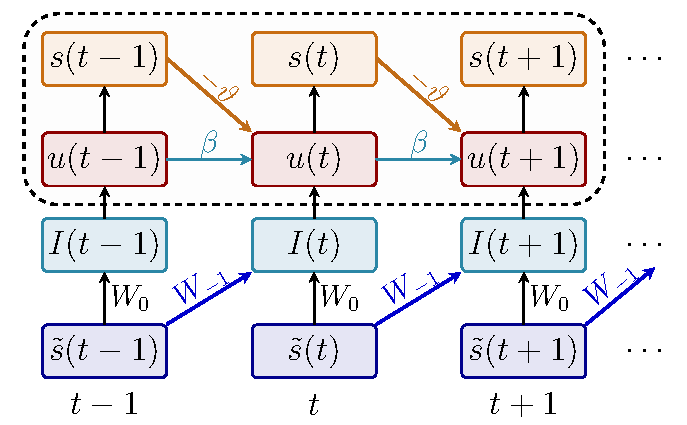
\includegraphics[width=\linewidth]{tikz_snntorch.pdf}%
  }
    \hfill
    \adjustbox{valign=c}{\includegraphics[width=0.49\textwidth]{pattern.pdf}}
  \caption{%
    Network architecture and a sample target motif. \emph{Left:}
    Unrolled view of the recurrent HD-SNN over time (one column representing one time step), illustrating delayed connections between neurons: Blue arrows indicate synaptic connections that integrate past activity across heterogeneous delays: the arrow labelled $\mathbf{W}$ stands for the weights over all $D$ delays. The context $\mathbf{c}(t)$ is the input received by the network at time $t$: the spike history over the $D$ previous steps, that is, the activity from $t-D$ to $t-1$ included ($t$ excluded), made of the target motif clamped during the trigger window, then the network's own recurrent spikes. Clamping input spikes is what excites the network: the trigger window is one such case, and other input spikes can be clamped in the same way. Once the trigger window is over, $\mathbf{c}(t)$ contains the spikes $s(t-1)$ emitted by the network itself, so that its output feeds back onto its input: this closes a recurrence loop, $s(t) \to \mathbf{c}(t+1) \to I(t+1) \to u(t+1) \to s(t+1)$, which the figure does not draw. The arrow labelled $-\vartheta$ depicts the subtractive reset of snnTorch, which subtracts the threshold from the membrane after each spike; the simulations reset the membrane to zero instead (Equation~\ref{eq:lif}), and the subtractive reset was one of the options scanned in Section~\ref{sec:hyperparameters}.
    \emph{Right:}
    One representative target spike motif, the second of the $M=16$ motifs, also shown in Figure~\ref{fig:target} ($N=1024$ neurons, $T=1000$ time steps); each red circle marks one target spike. The goal of the network is to memorise $M=16$ such motifs. Each trial is preceded by $50$ time steps of spontaneous background activity (random spikes at rate $p_A$) before the stimulus. The trigger window (green crosses between the dashed lines) consists of the first $D=41$ time steps of the target motif clamped to the network input; the recurrent network then autonomously predicts the remaining spikes.
  }\label{fig:model}
\end{figure}
%%%-----------------------------------------------------------------
